\section{Calibration Transport, Cost Crossovers, and Budget Curves}
\subsection{Cross-Age Calibration and Proper Scores}\label{app:transfer}
The protocol is fixed in \texttt{PROTOCOL\_v10.json}. Each of the 25 SAPA
targets uses the same twenty target-excluding features as the main
benchmark. We apply permutation seed 20261106 before dropping records
missing a selected feature, target, or age. The first 800 records fit the
depth-six tree with minimum leaf size 25 and tree seed 623. They belong
to neither calibration nor evaluation. Age at most 25 defines the younger
group and age above 25 the older group. Each group's first 500 remaining
records form its reference sample; its remaining 305--370 records define
the empirical evaluation law. Both directions are reported for every task.
The matched reference is an explicitly additional diagnostic resource,
not an assumed input to the source-reference audit. Conditional on the
frozen model, target-representative complete records permit direct
estimation whenever they are available.

We compare probability-matching accuracy, threshold accuracy, Brier
improvement and log-loss improvement clipped at 0.01 and 0.99. The loss
tables use the same frozen root and leaf probabilities in every condition.
Each target is constant on the same tree leaves, so branching calculates
it using at most six features. The form program uses all observed form
coordinates and separate constraints for each label. Its marginal
reference tables mix the 500-record frequencies with 0.1 times the uniform
law on each form--label space. This shrinkage and the probability floor
$q_T\ge0.1/L$ are fixed before evaluation, without target-population tuning.
No whole-profile enumeration is needed for this fit.

For every source-fitted and matched-fitted score we compute conditional
means and variances by exact finite sums over target records and random
form assignment. We also draw 1,000 independent audits of size 1,000 and
evaluate ordinary sample-variance Wald intervals. Numerical mean errors
and algebraic constraint residuals are released. Coverage summaries average
conditional simulations, with per-task Monte Carlo errors supplied; they
do not estimate deployment-level uncertainty from 50 independent cohorts.
Two thresholded tasks have identically zero contrasts in both directions
and are reported separately. All other task/metric/direction combinations
are included irrespective of the observed efficiency ratio.

\begin{table*}[t]
\centering
\caption{Calibration in both directions. Ratios are medians; coverage averages 1,000 simulated audits of size 1,000 per case. Source discrepancy is the median absolute difference of reference and evaluation means. Misses count source-reference intervals that omit the empirical target, a descriptive transport diagnostic.}
\label{tab:transferdetail}
\small
\setlength{\tabcolsep}{4pt}
\begin{tabular}{llrrrrrr}
\toprule
Metric & Direction & Cases & Matched & Shifted & Coverage & Discrepancy & Misses \\
\midrule
Randomized accuracy & $\le25\to>25$ & 25 & 2.542 & 2.548 & 0.950 & 0.0053 & 1/25 \\
Randomized accuracy & $>25\to\le25$ & 25 & 2.455 & 2.518 & 0.947 & 0.0082 & 8/25 \\
Threshold accuracy & $\le25\to>25$ & 23 & 1.049 & 1.056 & 0.949 & 0.0206 & 5/23 \\
Threshold accuracy & $>25\to\le25$ & 23 & 1.054 & 1.055 & 0.950 & 0.0220 & 10/23 \\
Brier improvement & $\le25\to>25$ & 25 & 2.372 & 2.351 & 0.951 & 0.0029 & 4/25 \\
Brier improvement & $>25\to\le25$ & 25 & 2.237 & 2.349 & 0.950 & 0.0049 & 5/25 \\
Clipped log loss & $\le25\to>25$ & 25 & 2.596 & 2.555 & 0.949 & 0.0143 & 3/25 \\
Clipped log loss & $>25\to\le25$ & 25 & 2.596 & 2.641 & 0.948 & 0.0181 & 4/25 \\
\bottomrule
\end{tabular}
\end{table*}


The source-reference direct mean is also reported as a transport diagnostic.
Its discrepancy from the target mean combines group differences and
finite reference/evaluation samples. Counting whether its conventional
500-record interval contains the empirical target is descriptive; it is
not a repeated-sampling coverage estimate for a population-level age effect.
Pointwise-unbiased form scores use source data only to choose variance,
and target audit records to estimate the target mean.

\subsection{Complete Records and Intermediate Label Cost}\label{app:cost10}
For fixed fitted scores and a common target population, let
$\sigma_F^2=\rho\sigma_B^2$ denote fixed and branching variances. Complete
records compute the branching target directly and have variance
$\sigma_B^2$. Ignoring the integer rounding of a planned sample size,
the ratio of total costs for equal variance is
\[
 \frac{C_F}{C_{\rm complete}}=\rho\frac{c_Y+b}{c_Y+m}.
\]
Solving its equality with one yields \eqref{eq:costcross}. If $\rho=1$
and $b<m$, the fixed design remains cheaper at every finite label cost;
if $m-b\rho\le0$, complete acquisition is weakly cheaper for all
nonnegative label costs. The released rows also use exact integer planning
counts $n_B,n_F$ and their crossover
$(mn_B-bn_F)/(n_F-n_B)$ whenever $n_F>n_B$.
The same-population complete-reference half-width is
$1.95996398454\sqrt{\sigma_B^2/500}$.

Complete acquisition is admissible only in the relaxed-cap comparison.
Randomly validating a subset of a larger enrolled cohort incurs a different
cost if labels are obtained on every enrollee. The residual-correction
comparator charges that cost explicitly; direct full-record sampling
enrols only the records it actually observes. This distinction is necessary
when label costs are substantial.

The all-task cost and precision calculations use all 70 existing frozen
score variances. Branching path lengths are recomputed from the same
frozen training protocol, with exact target-variance agreement checked.
Label costs are $0,1,3,10,30,100$. The ten-task correction diagnostic
reoptimizes its source-calibrated candidate forms, validation fractions and
within-form strata at $c_Y=10$, using the same candidate grid as
Appendix~\ref{app:validation}. Its new conditional coverage simulation has
2,000 audits per task. No calibration or pilot cost is silently included
in the per-record costs: the displayed comparisons condition on a supplied
reference, whereas Appendix~\ref{app:em} charges fresh capped calibration.

\begin{table*}[t]
\centering
\caption{All-task planned fixed-form/complete-record cost ratios at half-width 0.025. Counts include integer rounding and a minimum of 30. The last column counts tasks on which complete acquisition is cheaper. Both designs condition on supplied calibration.}
\label{tab:costdetail}
\small
\setlength{\tabcolsep}{4pt}
\begin{tabular}{lrrrr}
\toprule
Data & $c_Y$ & Tasks & Cost ratio & Complete cheaper \\
\midrule
SUSHI & 0 & 45 & 0.726 & 1/45 \\
SUSHI & 1 & 45 & 0.818 & 5/45 \\
SUSHI & 3 & 45 & 0.984 & 17/45 \\
SUSHI & 10 & 45 & 1.427 & 45/45 \\
SUSHI & 30 & 45 & 2.103 & 45/45 \\
SUSHI & 100 & 45 & 2.806 & 45/45 \\
SAPA & 0 & 25 & 0.731 & 3/25 \\
SAPA & 1 & 25 & 0.812 & 5/25 \\
SAPA & 3 & 25 & 0.953 & 11/25 \\
SAPA & 10 & 25 & 1.299 & 19/25 \\
SAPA & 30 & 25 & 1.754 & 25/25 \\
SAPA & 100 & 25 & 2.152 & 25/25 \\
\bottomrule
\end{tabular}
\end{table*}
\begin{table*}[t]
\centering
\caption{Intermediate-cost diagnostic at $c_Y=10$ on the ten fixed tasks. Validation is refitted at that cost, with 2,000 conditional coverage simulations per task. Other rows reuse verified variances.}
\label{tab:cost10detail}
\small
\setlength{\tabcolsep}{4pt}
\begin{tabular}{llrrr}
\toprule
Data & Method & Records & Cost & Validation coverage \\
\midrule
SAPA & branching & 104 & 1525 & -- \\
SAPA & complete & 104 & 3120 & -- \\
SAPA & debiased proxy & 108 & 3120 & 0.946 \\
SAPA & full form & 198 & 3168 & -- \\
SAPA & prefix & 246 & 3936 & -- \\
SUSHI & branching & 134 & 1994 & -- \\
SUSHI & complete & 134 & 5092 & -- \\
SUSHI & debiased proxy & 134 & 5092 & 0.948 \\
SUSHI & full form & 454 & 7264 & -- \\
SUSHI & prefix & 528 & 8448 & -- \\
\bottomrule
\end{tabular}
\end{table*}


\subsection{Identification Floors Across the Whole Budget Range}\label{app:budgetcurve}
We reuse the twenty binary12 prediction grids from
Appendix~\ref{app:nonlinear}, with no refitting or seed selection.
For each cap from zero to twelve, we seek feasible primal and dual
certificates for
$\delta_b=\inf_{\deg(v)\le b}\|d-v\|_\infty$.
The target comparison is with the fixed tolerance 0.025. Let $F_b$ contain
the degree-at-most-$b$ Walsh columns. When the complementary set is
smaller, an equivalent residual program minimizes $\|r\|_\infty$ subject
to $F_{>b}^{\mathsf T}r=F_{>b}^{\mathsf T}d$; then $d-r$ has degree at
most $b$. The code chooses the smaller coefficient representation.

Every LP has a 45-second solver limit. A feasible Fourier truncation and
its high-degree residual supply bounds if the optimizer does not finish.
Primal coefficients are rounded to multiples of $2^{-36}$. Rounded dual
vectors are projected exactly onto the high-degree Walsh subspace with
integer transforms. Exact rational evaluation against the released
binary64 targets gives certified endpoints, independently of solver status.
At cap twelve the identity approximation has zero error exactly. A narrow
bracket is not assumed when a solve reaches its time limit.

Because $\delta_b$ is nonincreasing, bounds from other budgets tighten
each bracket without changing its validity: the lower endpoint at $b$ is
the largest lower endpoint over budgets at least $b$, and its upper
endpoint is the smallest upper endpoint over budgets at most $b$.
For each task we report the last budget certified insufficient and the
first budget with an approximation residual strictly below 0.025.
Budgets between these endpoints are unresolved by the released
certificates. Crossing this approximation threshold permits, but does
not by itself provide, a finite-sample interval of that half-width.

\begin{table*}[t]
\centering
\caption{Certified bracket for the smallest cap with $\delta_b<0.025$. A lower endpoint $l$ means every cap below $l$ is certified insufficient; the upper endpoint has a feasible approximation below the tolerance. Equality identifies this minimum exactly.}
\label{tab:budgetthresholds}
\small
\setlength{\tabcolsep}{4pt}
\begin{tabular}{llrrr}
\toprule
Model & Output & Seed & Minimum cap LB & Minimum cap UB \\
\midrule
GBDT & probability & 20261108 & 4 & 5 \\
MLP & probability & 20261108 & 7 & 9 \\
GBDT & threshold & 20261108 & 6 & 6 \\
MLP & threshold & 20261108 & 10 & 10 \\
GBDT & probability & 20261109 & 4 & 5 \\
MLP & probability & 20261109 & 7 & 9 \\
GBDT & threshold & 20261109 & 7 & 9 \\
MLP & threshold & 20261109 & 10 & 10 \\
GBDT & probability & 20261110 & 4 & 6 \\
MLP & probability & 20261110 & 7 & 9 \\
GBDT & threshold & 20261110 & 8 & 9 \\
MLP & threshold & 20261110 & 10 & 10 \\
GBDT & probability & 20261111 & 4 & 5 \\
MLP & probability & 20261111 & 8 & 9 \\
GBDT & threshold & 20261111 & 7 & 7 \\
MLP & threshold & 20261111 & 10 & 10 \\
GBDT & probability & 20261112 & 4 & 5 \\
MLP & probability & 20261112 & 7 & 9 \\
GBDT & threshold & 20261112 & 7 & 9 \\
MLP & threshold & 20261112 & 10 & 10 \\
\bottomrule
\end{tabular}
\end{table*}
\begin{figure*}[t]
\centering
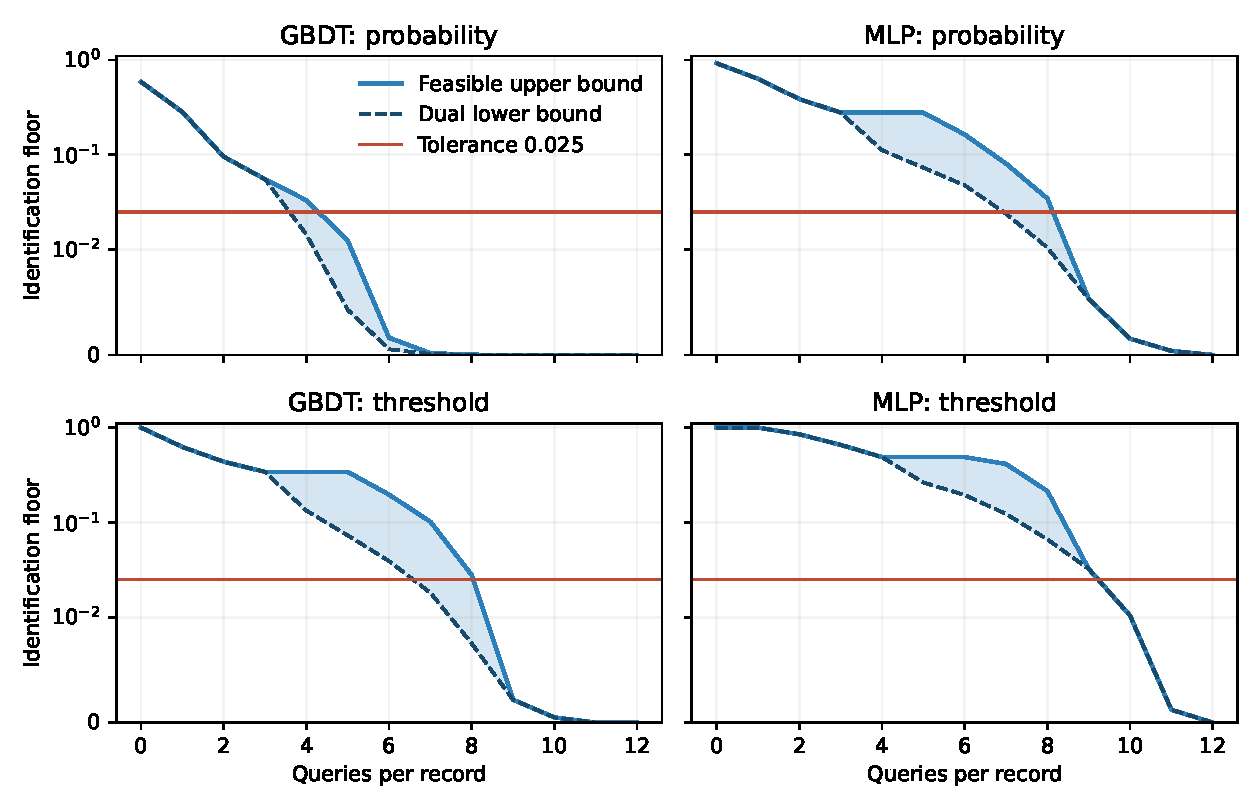
\includegraphics[width=.96\textwidth]{figures/budget_curves.pdf}
\caption{Median certified identification-floor brackets across five fixed WDBC splits. Solid curves are upper bounds, dashed curves lower bounds, and shading shows the remaining uncertainty. The horizontal line is the target 0.025. Upper and lower medians need not come from the same split. The vertical scale is linear below 0.01 and logarithmic above.}
\label{fig:budgetcurves}
\end{figure*}

